\chapter[Requisitos e Necessidade]{Requisitos e Necessidade}

Existem diversas técnicas de levantamento de requisitos, tradicionais ou modernas. Todas tem o objetivo de identificar os requisitos e diminuir problemas decorrentes durante uma má elicitação (CARVALHO).

Dentro do contexto de projetos de interação, exitem os \textit{storyboard}. São documentos utilizados, em maior peso, na industria de entretenimento audio-visual. Contem aspectos de detalhes da descrição visual (ORR). Com a utilização do \textit{storyboard} é possível descrever como o usuário se comportaria com a utilização do produto. Visando os aspectos como, qual a necessidade do usuário, possíveis reações com a utilização ou com a falta do produto, onde seria utilizado, entre outros.

A figura abaixo é um \textit{storyboard} passando a idéia central do contexto deste projeto. A história apresenta uma pessoa que está realizando a pesquisa de preços das passagens diversos  dias e horários, na sequência, tem o usuário preocupado, pois deveria estar procurando por preços mais em conta até que um dia apresentam esse aplicativo para ele e a partir dai ele pode ir dormir feliz e sem preocupações.

\begin{figure}[H]
	\centering
	\label{fig01}
		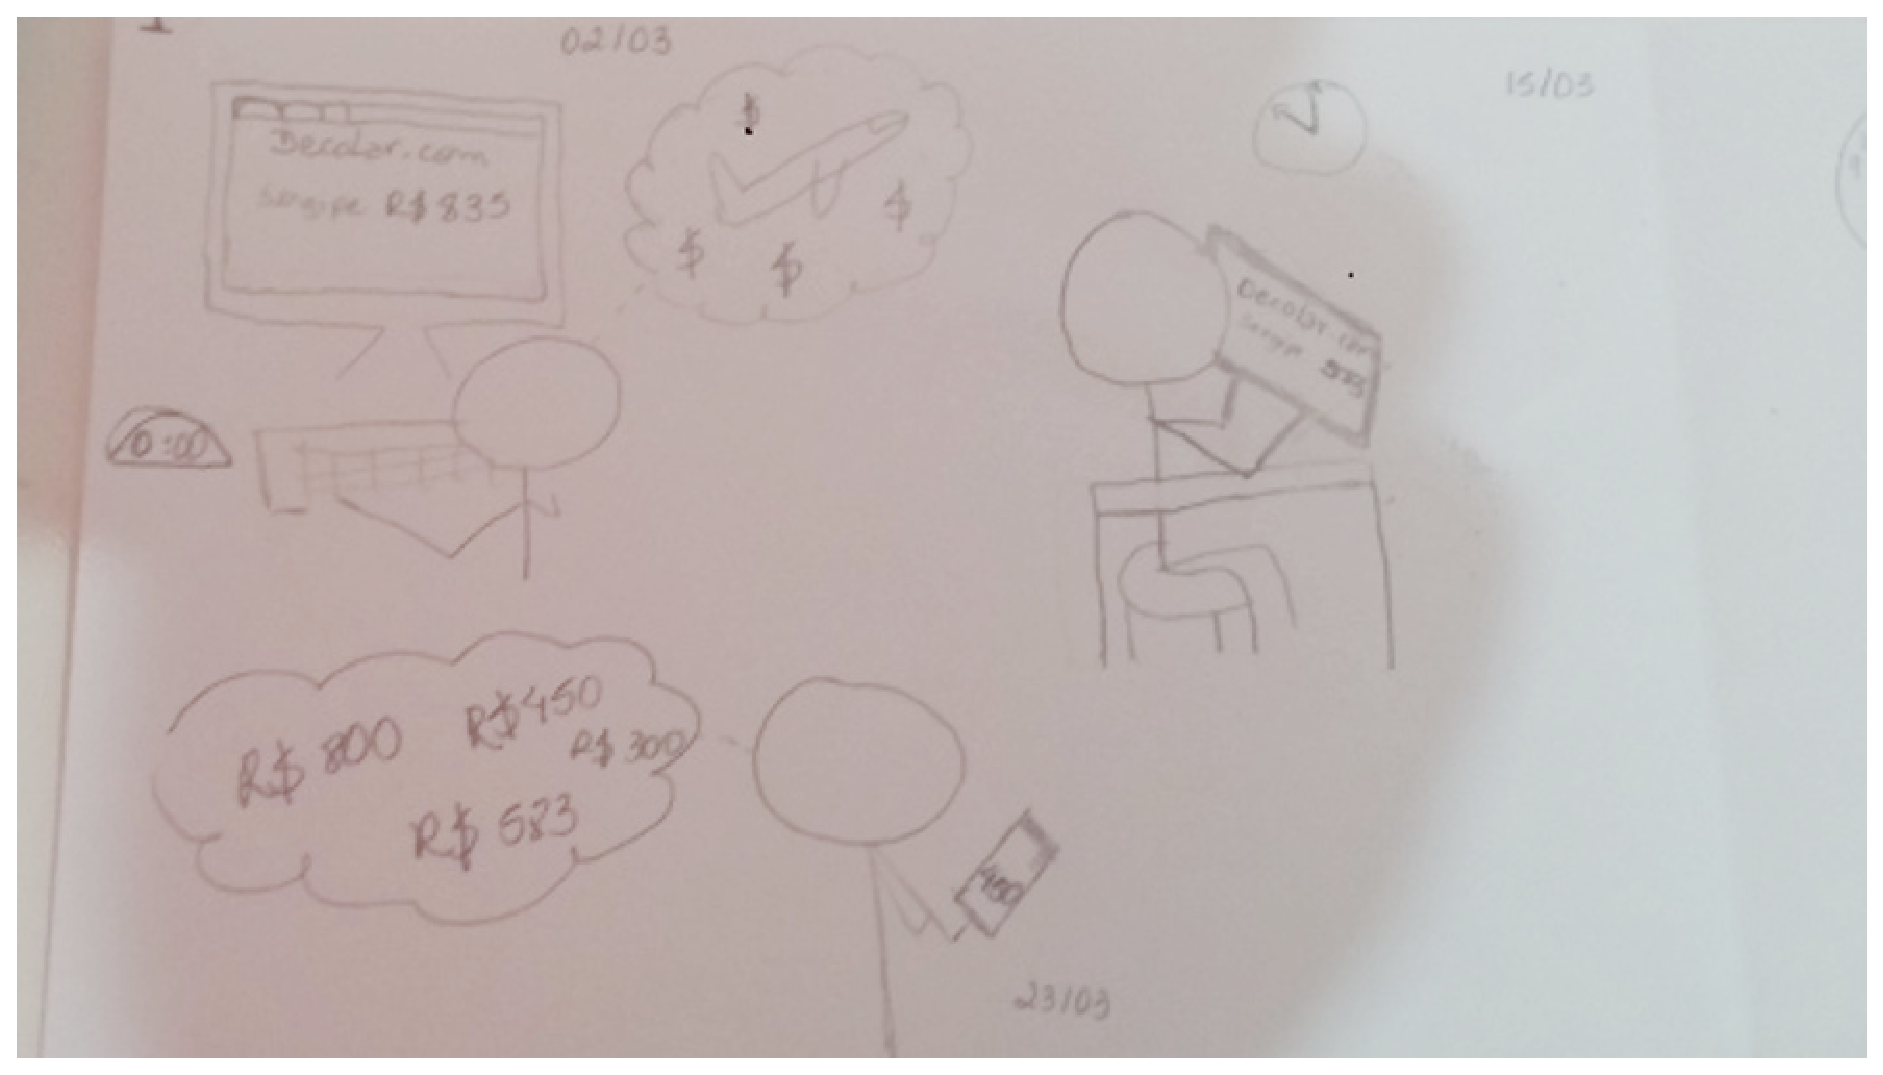
\includegraphics[keepaspectratio=true,scale=0.3]{figuras/quadro1.eps}
		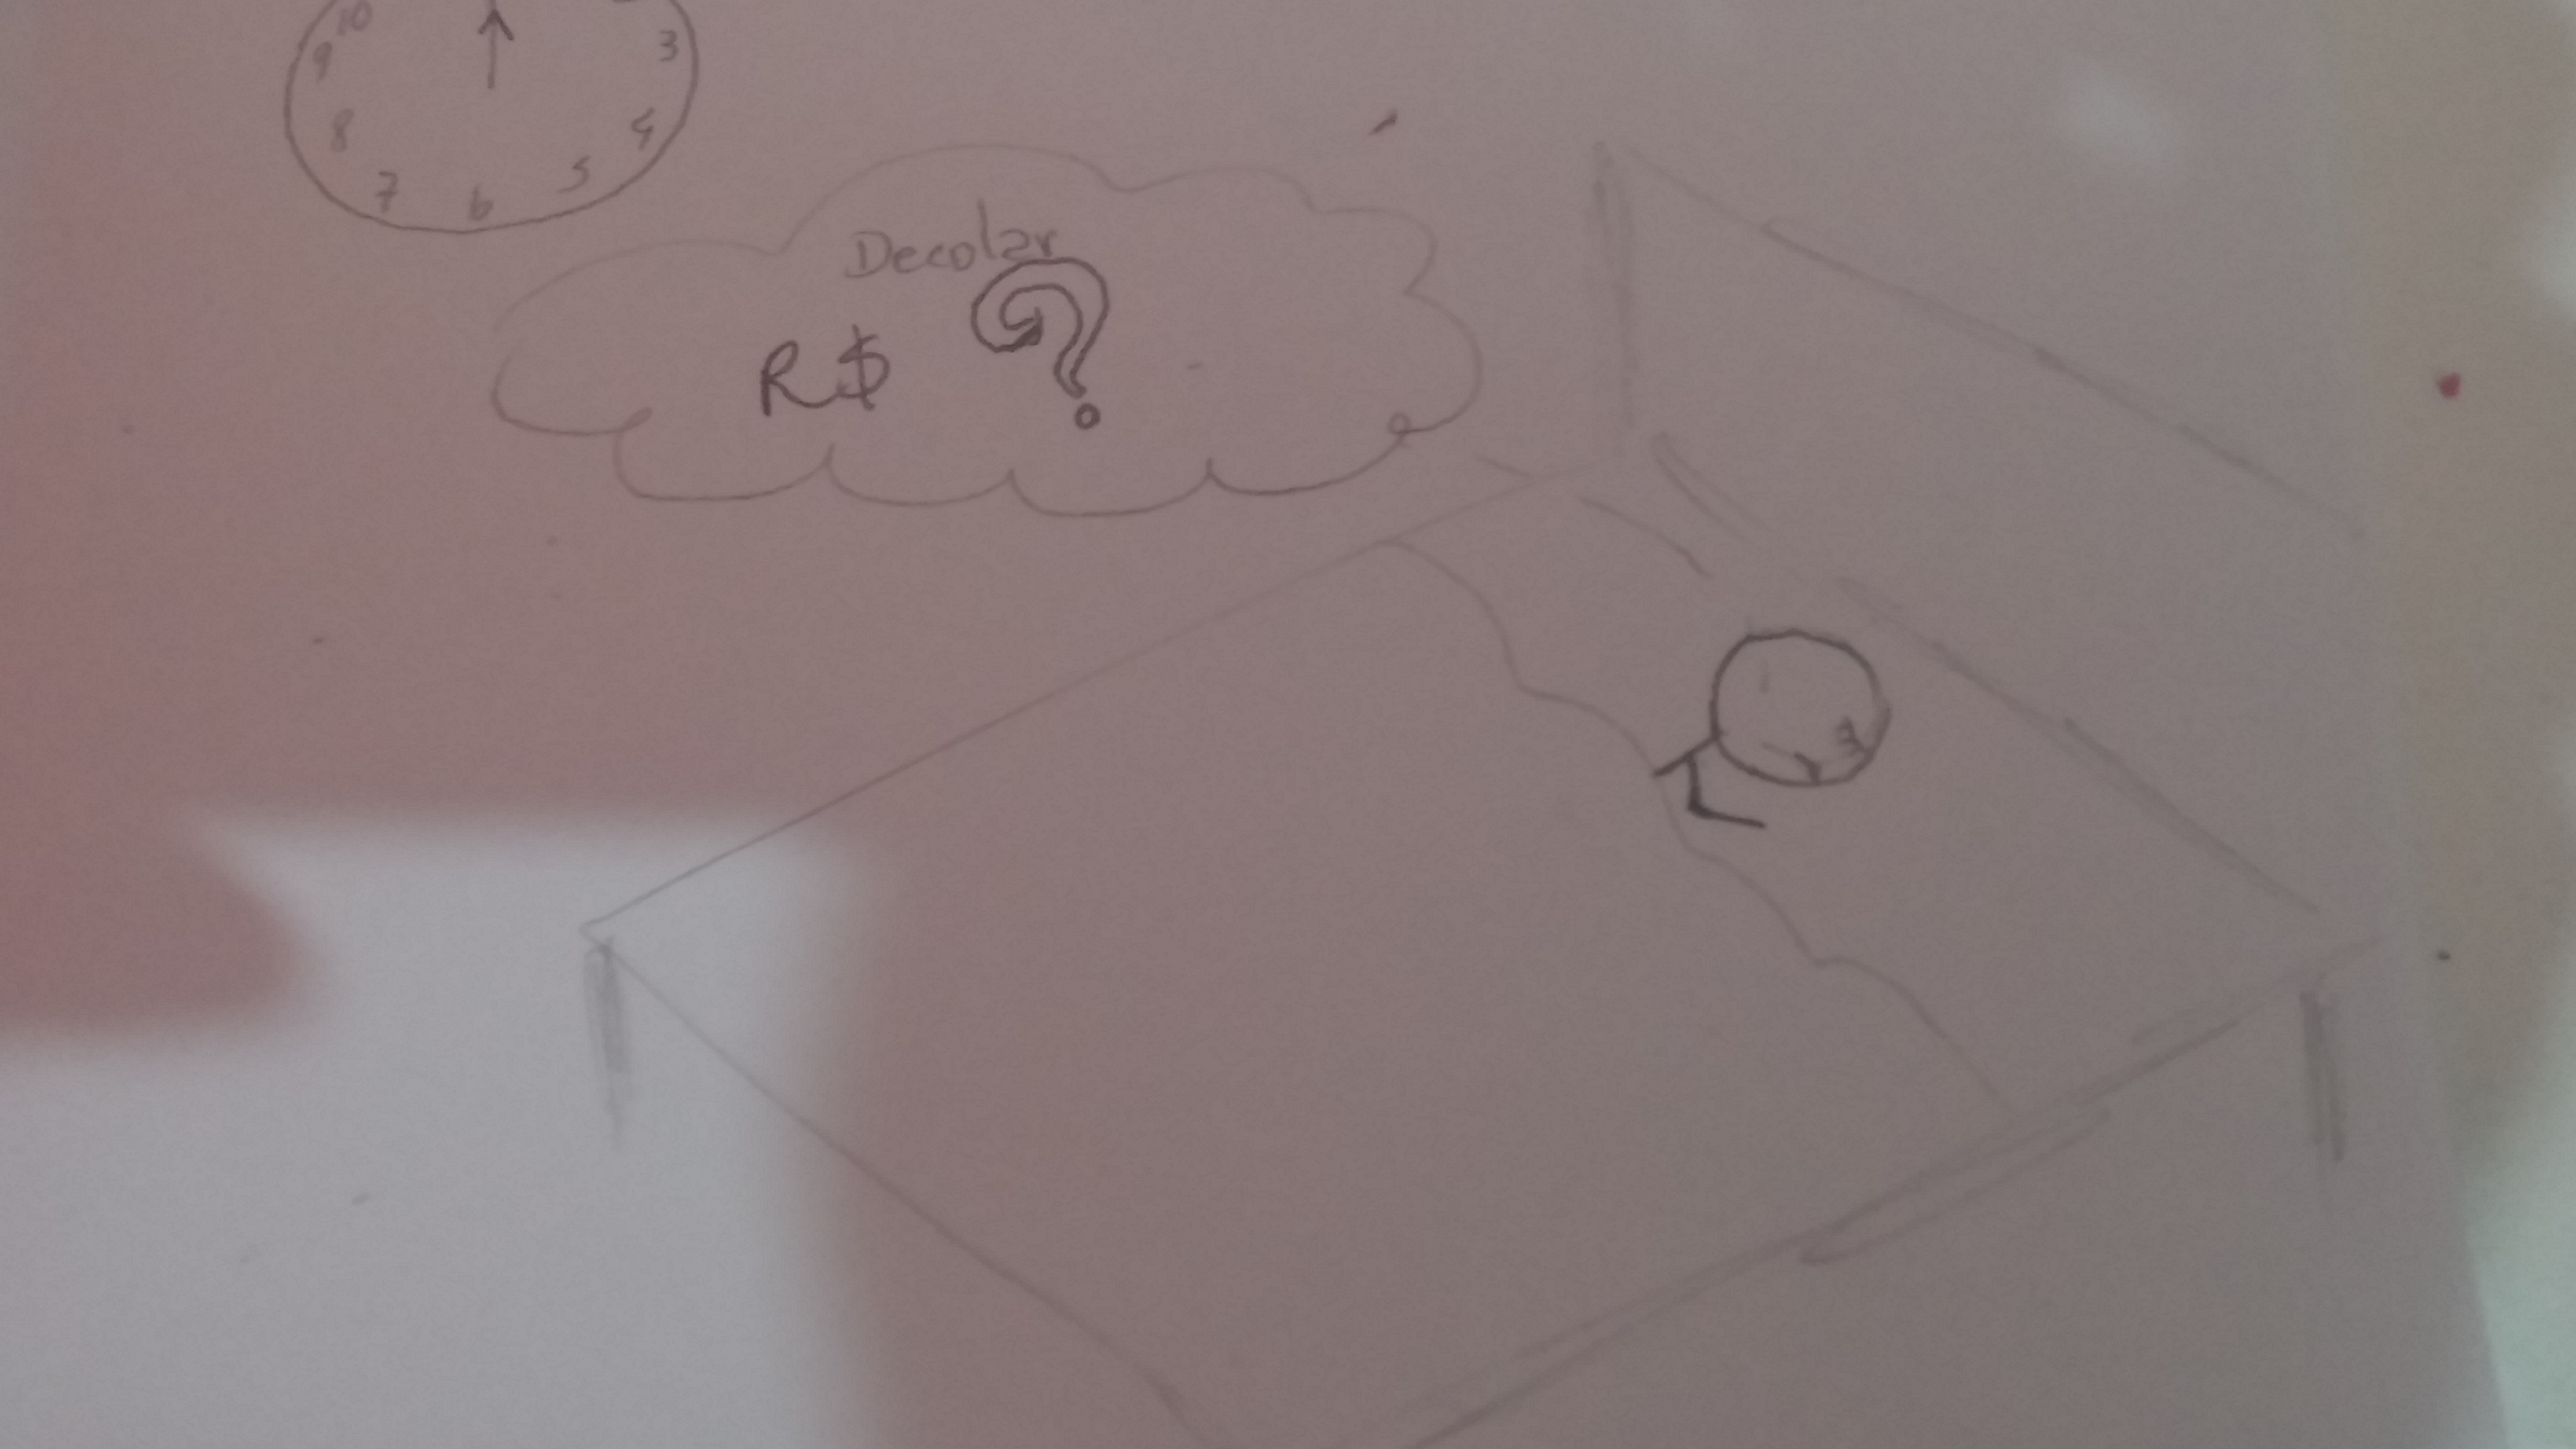
\includegraphics[keepaspectratio=true,scale=0.65]{figuras/quadro2.eps}
		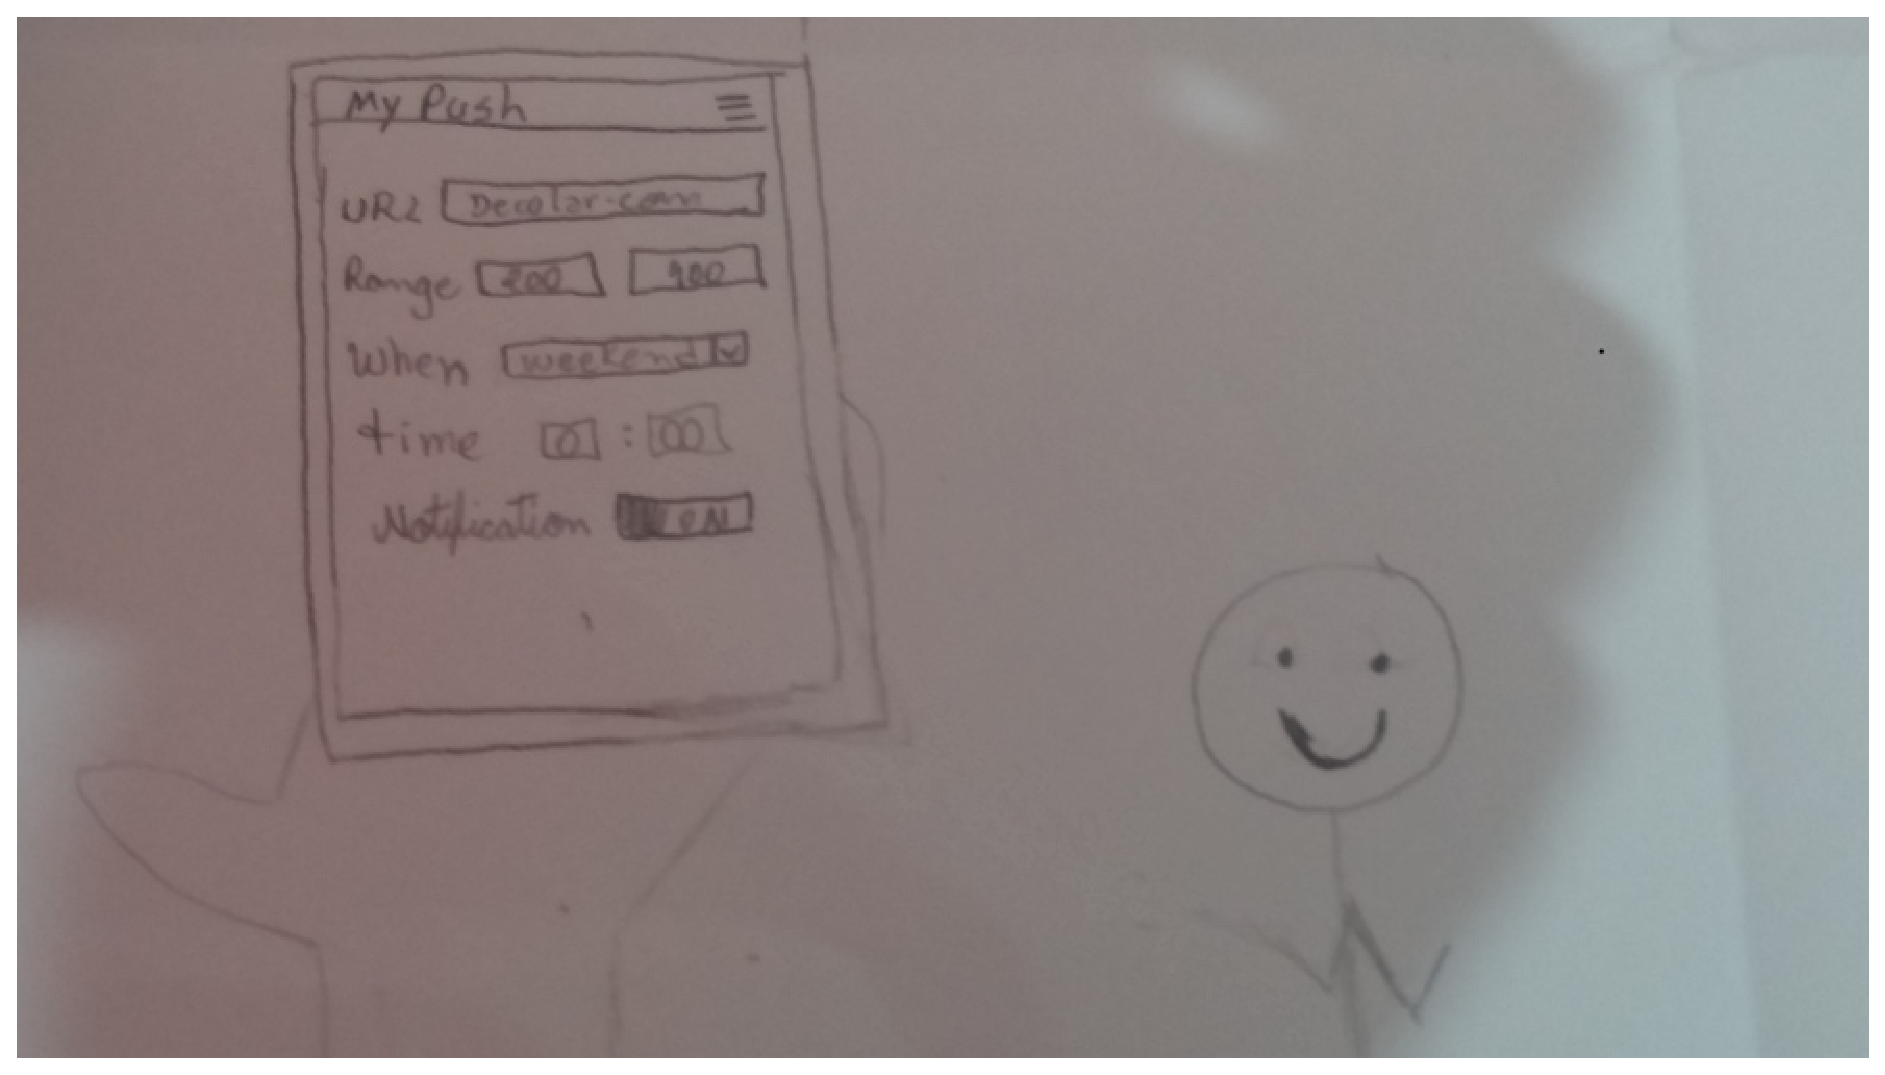
\includegraphics[keepaspectratio=true,scale=0.3]{figuras/quadro3.eps}
		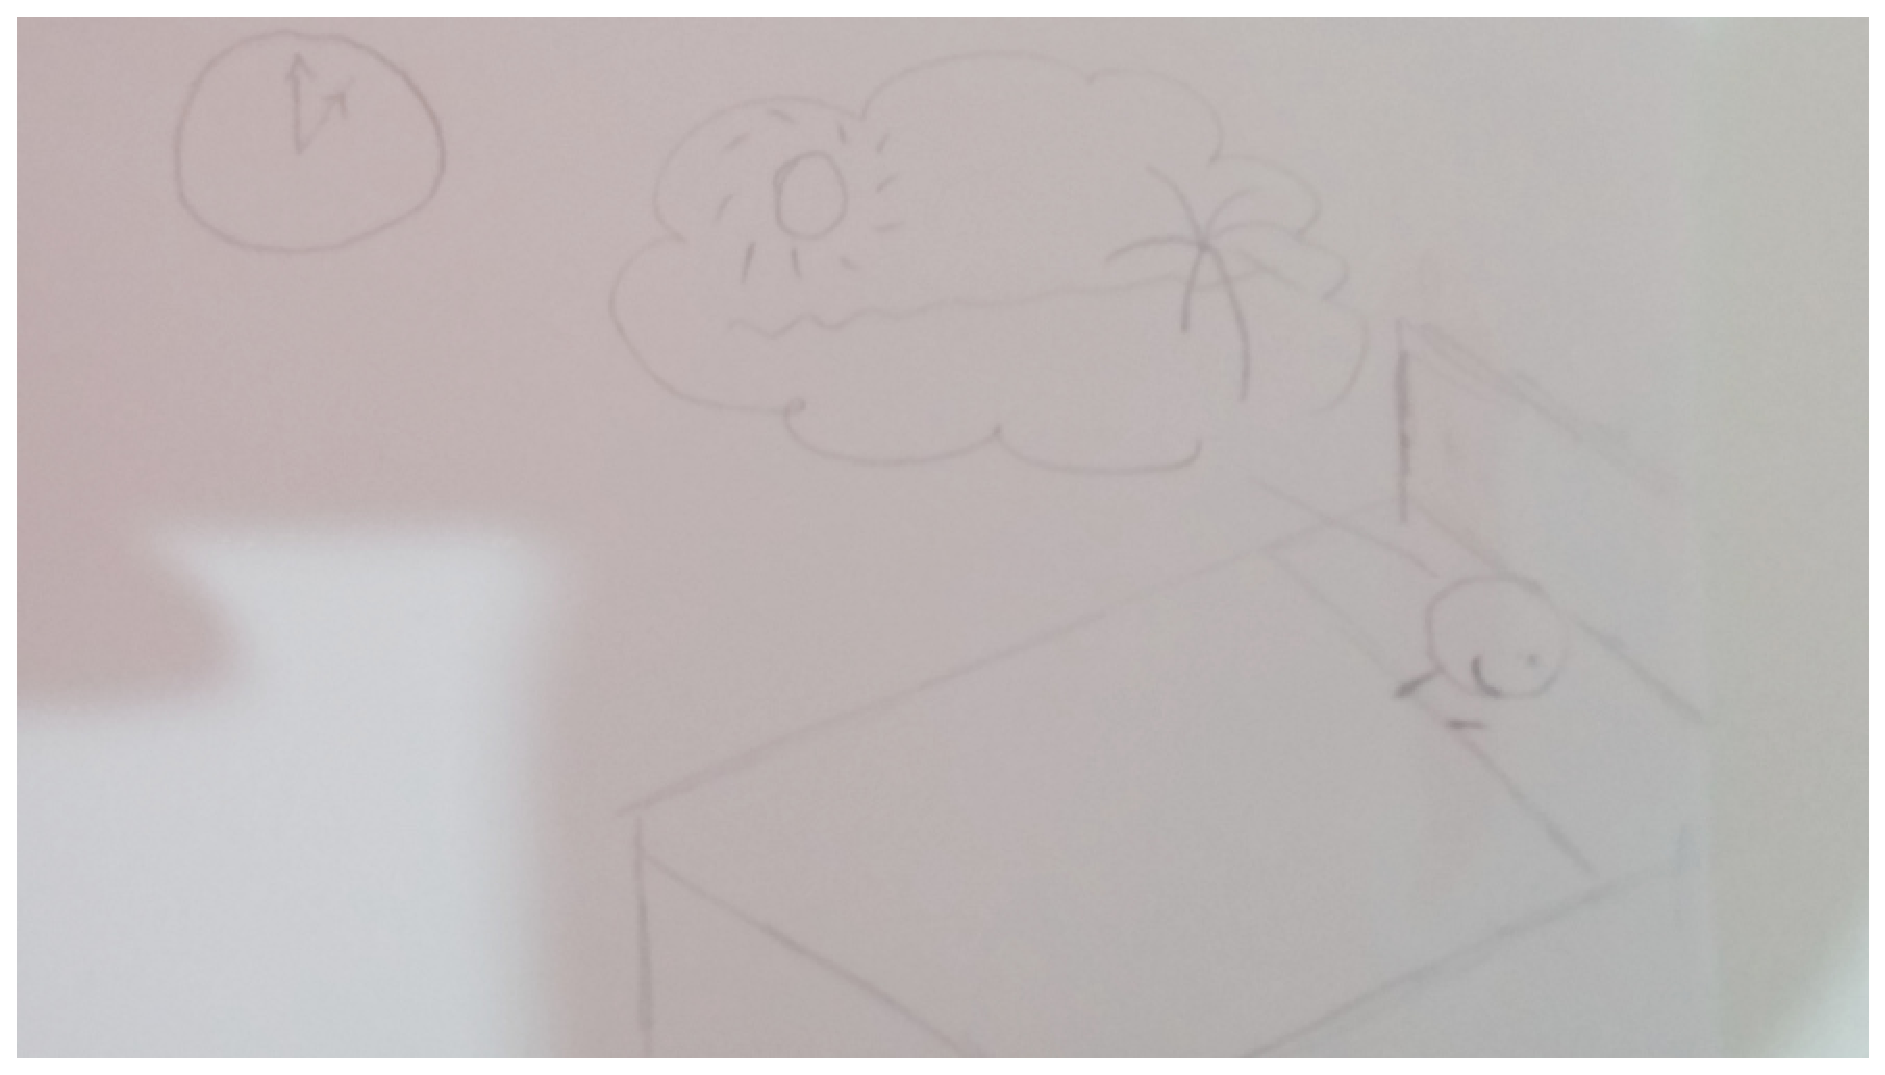
\includegraphics[keepaspectratio=true,scale=0.3]{figuras/quadro4.eps}
	\caption{Story Board - papel}
\end{figure}

\begin{figure}[H]
	\centering
	\label{fig02}
		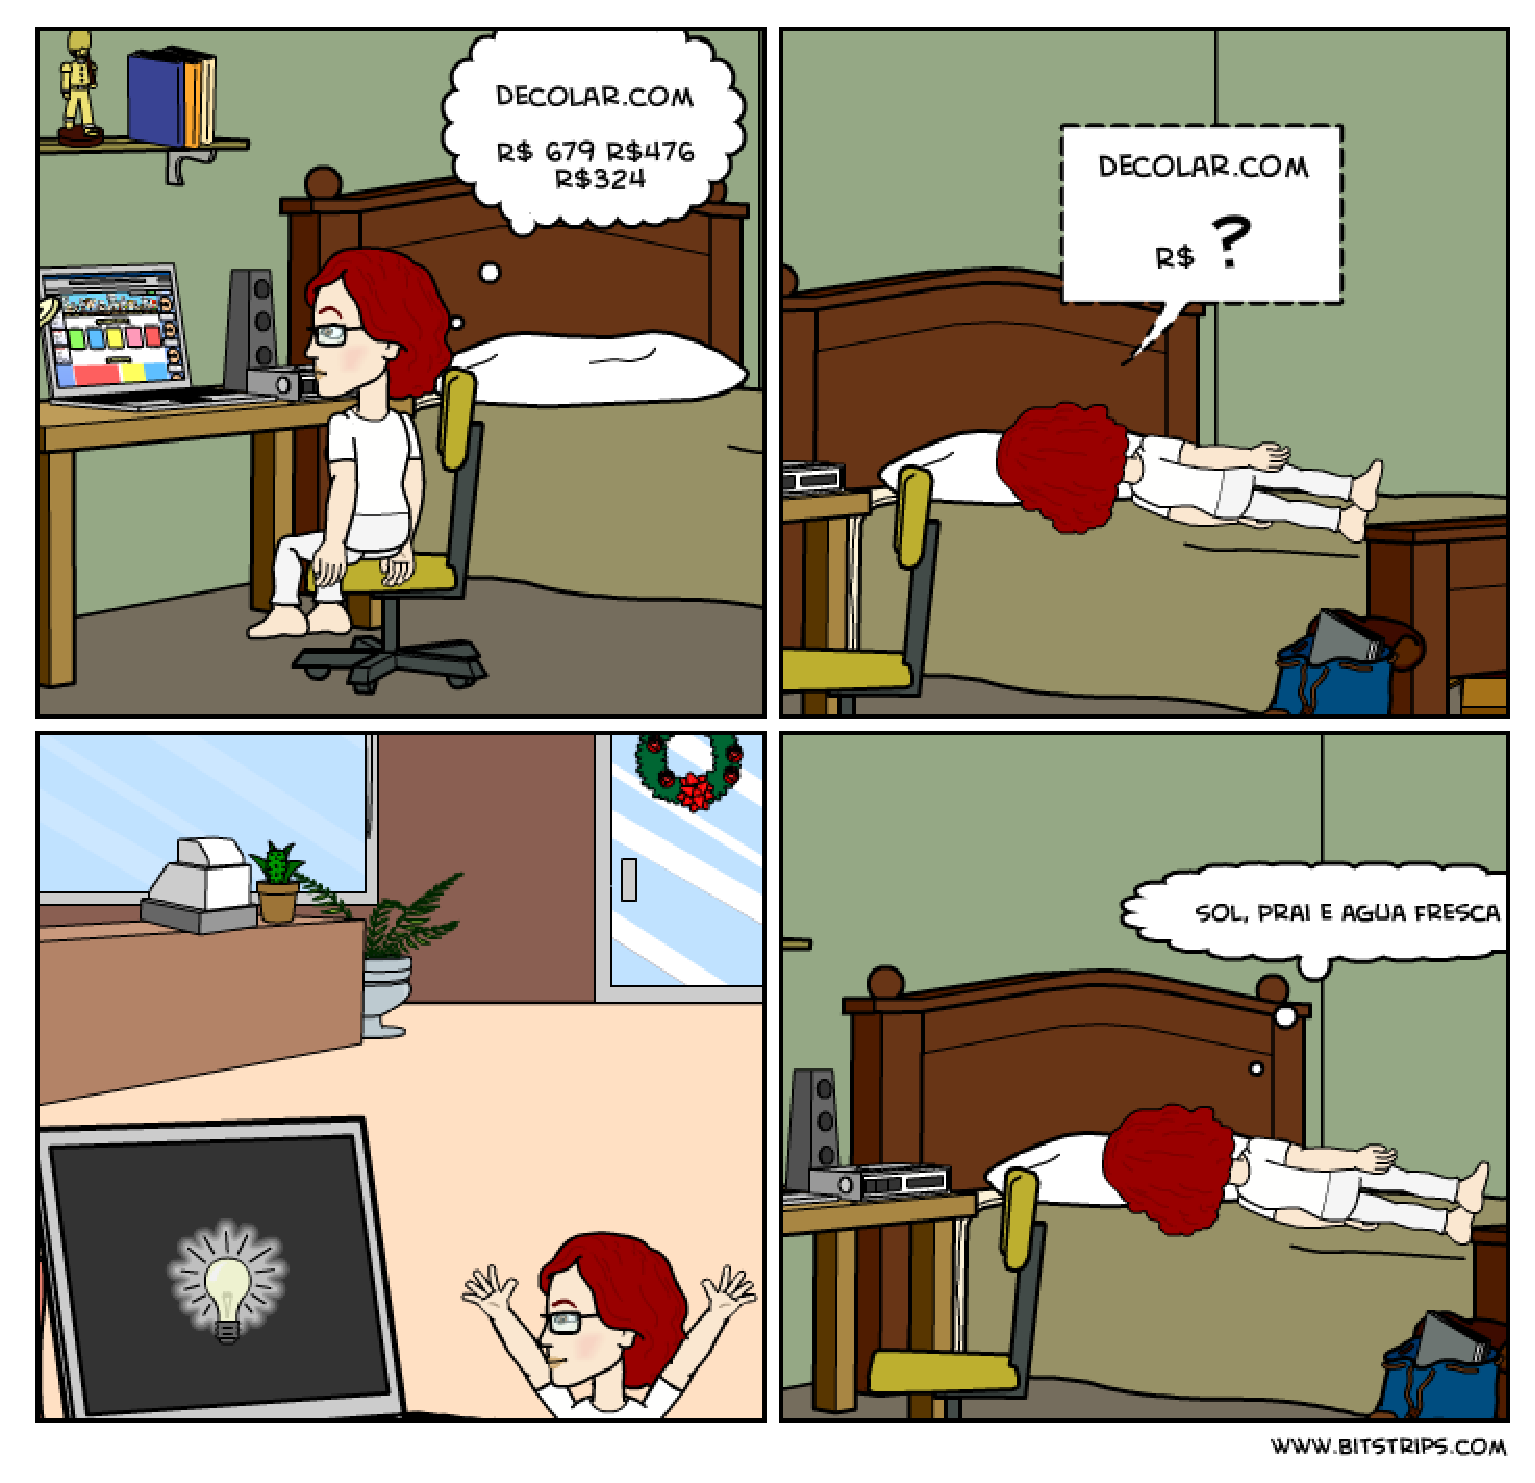
\includegraphics[keepaspectratio=true,scale=0.5]{figuras/ferramenta.eps}
		\caption{Story Board - ferramenta}
\end{figure}

Tendo como base o \textit{storyboard} é possível estabelecer as necessidades do usuário. Nesse contexto é possível retirar:

\begin{itemize}
	\item É de necessidade do usuário um sistema automatizado para realizar pesquisas de preços de passagens aéreas que seja simples de ser utilizar para diminuir o esforço nessa procura e não perder eventuais promoções das companias.
\end{itemize}

\section{Requisitos}

Os requisitos podem ser divididos em varias categorias (BLASCHEK, 2002), mas as de maior impacto para o projeto são:
\begin{itemize}
	\item \textbf{Funcionais}: o que o sistema deve realizar para que o usuário execute a atividade para alcançar o objetivo de negócio;
	\item \textbf{Não-Funcionais}: padrões e regulamentos com os quais restrigem os requisitos funcionais.
\end{itemize}

\subsection{Funcionais}

A partir do contexto de negócio e do levantamento do \textit{storyboard} da aplicação, foi construido a tabela abaixo que mostra os requisitos funcionais do sistema, cada qual com a sua identificação, descrição e prioridade (determinada pelo modelo do negócio).

\begin{table}[h]
	\centering
	\begin{tabular}{p{3cm}|p{7cm}|p{4cm}}
		\toprule
			\textbf{Id} & \textbf{Descrição} & \textbf{Prioridade} \\ \hline
		\midrule
			RF01 & O sistema deve ter um histórico contendo os acessos as passagens feito pelo usuário & Média \\ \hline
			RF02 & O sistema deve ter um lista ordenada das passagens mais baratas disponíveis no dia & Alta \\ \hline
			RF03 & O sistema deve ter um gráfico por meses mostrando o comportamento dos preços das passagens naquele mês & Alta \\ \hline
			RF04 & O sistema deve permitir inserir o site de vendas de passagens aéreas & Alta \\ \hline
			RF05 & O sistema deve permitir inserir nas configurações de notificação um filtro para o intervalo de preço que ele deseja receber & Alta \\ \hline
			RF06 & O sistema deve permitir configurar a data e hora específica para a notificação dos preços & Alta \\ \hline
			RF07 & O sistema deve permitir exportar o histórico de acesso aos preços das passagens em formato PDF & Média \\ \hline
			RF08 & O sistema deve permitir configurar a notificação para que ele receba no exato momento em que a promoção for lançada & Média \\ \hline
		\bottomrule
	\end{tabular}
	\caption{Requisitos funcionais do sistema MyPush Travel}
	\label{tab01}
\end{table}

\subsection{Não Funcionais}

A tabela abaixo mostra os requisitos não-funcionais levantados para o projeto MyPush Travel:

\begin{table}[H]
	\centering
	\begin{tabular}{p{3cm}|p{5cm}|p{6cm}}
		\toprule
			\textbf{Id} & \textbf{Tipo} & \textbf{Descrição} \\ \hline
		\midrule
			RNF01 & Usabilidade & O sistema deve apresentar uma mensagem caso os preços não se adequem as configurações durante o período de 15 dias \\ \hline
			RNF02 & Usabilidade & O sistema deve ser responsivo, se adequando a diferentes telas de smartphones \\ \hline
			RNF03 & Confiabilidade & O sistema deve realizar o backup do histórico de preços \\ \hline
			RNF04 & Confiabilidade & O sistema deverá guardar o backup do histórico de preços por um ano \\ \hline
			RNF05 & Confiabilidade & O sistema deverá fazer consultas no site informado somente nos dias e horários configurados \\ \hline
			RNF06 & Suportabilidade & O sistema deverá ser compatível com a plataforma android a partir da versão 2.3.3 \\ \hline
			RNF07 & Projeto & O sistema deverá usar o banco sqlite \\ \hline
		\bottomrule
	\end{tabular}
	\caption{Requisitos não-funcionais do sistema MyPush Travel}
	\label{tab02}
\end{table}

\section{Casos de Uso}

Com base no levantamento acima, teve-se um arranjo dos requisitos para a formação dos casos de uso do sistema. A figura abaixo mostra o diagrama e em seguida uma tabela com a descrição e associação dos requisitos de cada.

\begin{figure}[H]
	\centering
	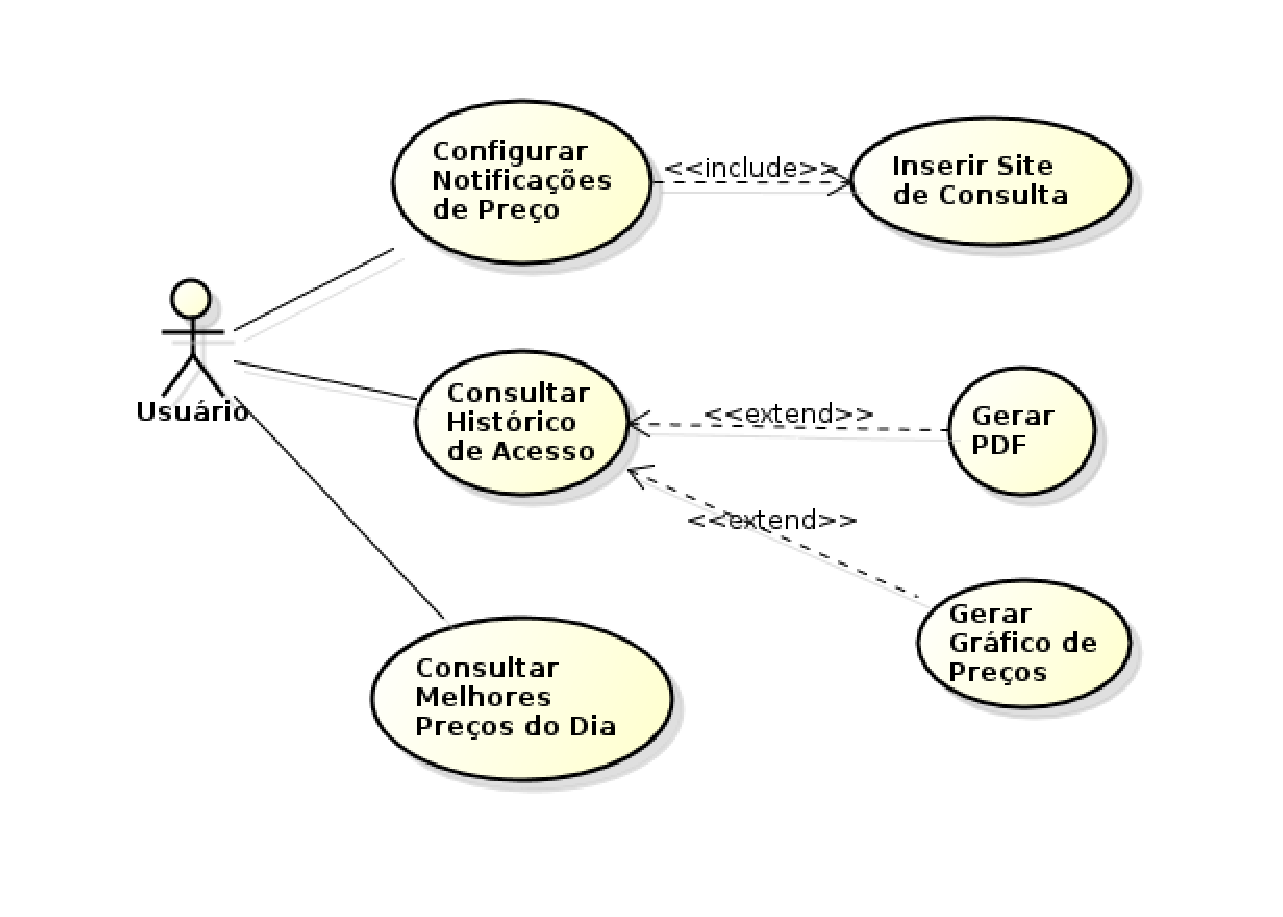
\includegraphics[scale=0.5]{figuras/caso_de_uso_mypush.eps}
	\caption{Diagrama de caso de uso do sistema MyPush Travel}
\end{figure}

\begin{table}[H]
	\centering
	\begin{tabular}{p{3cm}|p{4cm}|p{4cm}|p{3cm}}
		\toprule
			\textbf{Id} & \textbf{Caso de Uso} & \textbf{Descrição} & \textbf{Requisitos} \\ \hline
		\midrule
			CU01 & Configurar Notificações de Preço & Configura o dia, hora, preço e quais sites aparecerão nas notificações diárias & RF05, RF06, RF08 \\ \hline
			CU02 & Inserir Site de Consulta & Insere um site válido para que receba notificações contendo informações dele & RF04 \\ \hline
			CU03 & Consultar Histórico de Acesso & Mostra o histórico de quais preços, companias ou sites o usuário visitou & RF01, RF07 \\ \hline
			CU04 & Gerar Gráfico do Preços & Mostra um gráfico filtrado por mês dos preços das companias selecionadas & RF03 \\ \hline
			CU05 & Consultar Melhores Preços do Dia & Mostra uma lista dos melhores preços do dia de todas as companias & RF02 \\ \hline
		\bottomrule
	\end{tabular}
	\caption{Casos de uso do sistema MyPush Travel}
	\label{tab03}
\end{table}